\documentclass[12pt, a4paper]{article}
\usepackage{../../../myconfig} % Gọi file cấu hình từ ngoài gốc vào

% ==========================================
% BẮT ĐẦU NỘI DUNG TÀI LIỆU
% ==========================================
\begin{document}

% Truyền 3 tham số: {Nhãn cam} {Chữ to chính giữa} {Chữ ở góc phải Header}
\titlebox{KTDK}{Đề kiểm tra định kỳ lần 8}{Kiểm tra định kỳ}

\textit{\textbf{Phần I: Thí sinh trả lời từ câu 1 đến câu 12, mỗi câu thí sinh chỉ chọn một phương án}}

\vspace{0.5cm}
% --- CÂU 1 ---
\questionLinesManual{0}{1}{Cho tứ diện \(ABCD\). Gọi \(M\) và \(P\) lần lượt là trung điểm của các cạnh \(AB\) và \(CD\). Đặt \(\vec{BA} = \vec{b}, \vec{AC} = \vec{c}, \vec{AD} = \vec{d}\). Khẳng định nào sau đây đúng?}{%
    \begin{tasks}(2)
        \task \(\vec{MP} = \dfrac{1}{2}\left( \vec{c} + \vec{d} + \vec{b} \right)\)
        \task \(\vec{MP} = \dfrac{1}{2}\left( \vec{d} + \vec{b} - \vec{c} \right)\)
        \task \(\vec{MP} = \dfrac{1}{2}\left( \vec{c} + \vec{b} - \vec{d} \right)\)
        \task \(\vec{MP} = \dfrac{1}{2}\left( \vec{c} + \vec{d} - \vec{b} \right)\)
    \end{tasks}
}

% --- CÂU 2 ---
\questionLinesManual{0}{2}{Trong không gian \(Oxyz\), cho ba vectơ \(\vec{a} = (3; 0; 1), \vec{b} = (2; 1; -1)\) và \(\vec{c} = \vec{i} -\vec{j}-2\vec{k}\). Tích vô hướng \(\vec{a}\left( \vec{b} + \vec{c} \right)\) bằng}{%
    \begin{tasks}(4)
        \task 0
        \task 3
        \task 6
        \task 9
    \end{tasks}
}

% --- CÂU 3 ---
\questionLinesManual{0}{3}{Trong không gian với hệ tọa độ \(Oxyz\), cho hai vectơ \(\vec{m} = (1; 1; 4), \vec{n} = (4; 1; 1)\). Vectơ nào dưới đây vuông góc với cả hai vectơ \(\vec{m}\) và \(\vec{n}\)?}{%
    \begin{tasks}(4)
        \task \(\vec{a} = (1; 5; 1)\)
        \task \(\vec{b} = (1; -5; 1)\)
        \task \(\vec{c} = (1; 5; -1)\)
        \task \(\vec{d} = (-1; 5; 1)\)
    \end{tasks}
}

% --- CÂU 4 ---
\questionLinesManual{0}{4}{Trong không gian \(Oxyz\), cho mặt cầu \((S)\) có tâm \(I(0; -2; 1)\) và bán kính \(R = 5\). Phương trình của \((S)\) là}{%
    \begin{tasks}(2)
        \task \(x^2 + (y + 2)^2 + (z - 1)^2 = 25\)
        \task \(x^2 + (y - 2)^2 + (z + 1)^2 = 25\)
        \task \(x^2 + (y + 2)^2 + (z - 1)^2 = 5\)
        \task \(x^2 + (y - 2)^2 + (z + 1)^2 = 5\)
    \end{tasks}
}

% --- CÂU 5 ---
\questionLinesManual{0}{5}{Trong không gian \(Oxyz\), phương trình đường thẳng đi qua điểm \(A(1; 2; 3)\) và song song với đường thẳng \(d: \begin{cases} x = 1 - t \\ y = t \\ z = -1 - 4t \end{cases}\) là}{%
    \begin{tasks}(2)
        \task \(\dfrac{x-1}{-1} = \dfrac{y+2}{1} = \dfrac{z+3}{-4}\)
        \task \(\dfrac{x-1}{-1} = \dfrac{y+2}{1} = \dfrac{z-3}{-4}\)
        \task \(\dfrac{x-1}{1} = \dfrac{y-2}{1} = \dfrac{z-3}{4}\)
        \task \(\dfrac{x}{1} = \dfrac{y-3}{-1} = \dfrac{z+1}{4}\)
    \end{tasks}
}

% --- CÂU 6 ---
\questionLinesManual{0}{6}{Trong không gian \(Oxyz\), mặt phẳng qua \(A(1; 2; -1)\) và vuông góc với các mặt phẳng \((P): 2x - y + 3z - 2 = 0\); \((Q): x + y + z - 1 = 0\) có phương trình là}{%
    \begin{tasks}(2)
        \task \(x + y + 2z - 1 = 0\)
        \task \(4x - y + z - 1 = 0\)
        \task \(4x - y - 3z - 5 = 0\)
        \task \(x - y + z + 2 = 0\)
    \end{tasks}
}

% --- CÂU 7 ---
\questionLinesManual{0}{7}{Cho hình lập phương \(ABCD.A'B'C'D'\) có cạnh bằng 4. Tính tích vô hướng \(\vec{AC'} \cdot \vec{BC}\).

\begin{center}
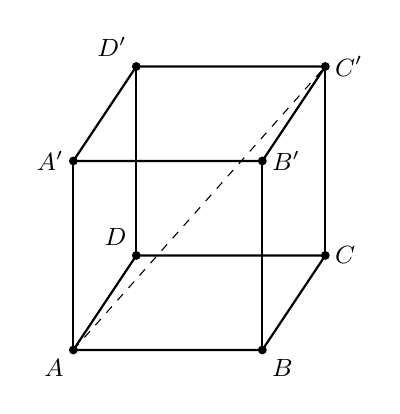
\begin{tikzpicture}[>=latex, scale=0.8]
    % 1. Vẽ hình lập phương
    \coordinate (A) at (0,0);
    \coordinate (B) at (3,0);
    \coordinate (C) at (4,1.5);
    \coordinate (D) at (1,1.5);
    \coordinate (A') at (0,3);
    \coordinate (B') at (3,3);
    \coordinate (C') at (4,4.5);
    \coordinate (D') at (1,4.5);
    
    % 2. Vẽ các cạnh
    \draw[thick] (A) -- (B) -- (C) -- (D) -- cycle;
    \draw[thick] (A') -- (B') -- (C') -- (D') -- cycle;
    \draw[thick] (A) -- (A');
    \draw[thick] (B) -- (B');
    \draw[thick] (C) -- (C');
    \draw[thick] (D) -- (D');
    
    % 3. Vẽ các đường chéo (nét đứt)

    \draw[dashed] (A) -- (C');
    
    % 4. Đánh dấu các đỉnh
    \fill (A) circle (2pt);
    \node[below left] at (A) {\small $A$};
    \fill (B) circle (2pt);
    \node[below right] at (B) {\small $B$};
    \fill (C) circle (2pt);
    \node[right] at (C) {\small $C$};
    \fill (D) circle (2pt);
    \node[above left] at (D) {\small $D$};
    \fill (A') circle (2pt);
    \node[left] at (A') {\small $A'$};
    \fill (B') circle (2pt);
    \node[right] at (B') {\small $B'$};
    \fill (C') circle (2pt);
    \node[right] at (C') {\small $C'$};
    \fill (D') circle (2pt);
    \node[above left] at (D') {\small $D'$};
    
\end{tikzpicture}
\end{center}
}{%
    \begin{tasks}(4)
        \task \(8\sqrt{3}\)
        \task \(16\sqrt{3}\)
        \task 16
        \task 0
    \end{tasks}
}

% --- CÂU 8 ---
\questionLinesManual{0}{8}{Trong mặt phẳng \(Oxy\), tâm của đường tròn \((C): x^2 + y^2 + 6x - 4y - 23 = 0\) có tọa độ là}{%
    \begin{tasks}(4)
        \task \((-3; 2)\)
        \task \((3; 2)\)
        \task \((3; -2)\)
        \task \((-3; -2)\)
    \end{tasks}
}

% --- CÂU 9 ---
\questionLinesManual{0}{9}{Trong không gian \(Oxyz\), điểm \(A'\) đối xứng với điểm \(A(2; -3; 1)\) qua mặt phẳng \(Oxz\) có tọa độ là}{%
    \begin{tasks}(4)
        \task \((-2; 3; -1)\)
        \task \((-2; -3; 1)\)
        \task \((2; -3; -1)\)
        \task \((2; 3; 1)\)
    \end{tasks}
}

% --- CÂU 10 ---
\questionLinesManual{0}{10}{Trong không gian với hệ trục tọa độ \(Oxyz\), cho mặt phẳng \((P)\) đi qua \(O\) và có vectơ pháp tuyến \(\vec{n} = (2; -2; 1)\). Khoảng cách từ điểm \(M(3; -1; 1)\) đến \((P)\) bằng}{%
    \begin{tasks}(4)
        \task 3
        \task \(\dfrac{5}{3}\)
        \task 1
        \task 9
    \end{tasks}
}

% --- CÂU 11 ---
\questionLinesManual{0}{11}{Trong không gian với hệ trục tọa độ \(Oxyz\), cho hai vector \(\vec{a} = (1; -2; 1)\), \(\vec{b} = (-2; 1; 1)\). Góc giữa hai vector \(\vec{a}\) và \(\vec{b}\) là}{%
    \begin{tasks}(4)
        \task \(30^\circ\)
        \task \(120^\circ\)
        \task \(60^\circ\)
        \task \(150^\circ\)
    \end{tasks}
}

% --- CÂU 12 ---
\questionLinesManual{0}{12}{Trong không gian \(Oxyz\), điểm nào sau đây thuộc đường thẳng \(d: \dfrac{x-1}{1} = \dfrac{y}{2} = \dfrac{z+1}{-2}\)?}{%
    \begin{tasks}(4)
        \task \(N(1; 2; -2)\)
        \task \(P(-1; 0; 1)\)
        \task \(Q(2; 1; -2)\)
        \task \(M(1; 0; -1)\)
    \end{tasks}
}

\newpage

\textit{\textbf{Phần II: Thí sinh trả lời từ câu 13 đến câu 16; trong mỗi ý a), b), c), d) ở mỗi câu, thí sinh chọn đúng hoặc sai.}}

\vspace{0.3cm}

% --- CÂU 13 ---
\questionTrueFalse{0}{13}{Trong không gian \(Oxyz\), cho hai điểm \(A(1; 2; 3)\), \(B(-2; 0; 1)\) và đường thẳng \(\Delta: \begin{cases} x = 1 + 2t \\ y = -3t \\ z = t - 1 \end{cases} (t \in \mathbb{R})\). Gọi \(N\) là điểm thuộc \(\Delta\).}{
    \textbf{a)} & Khi góc \(\widehat{ABN}\) là góc tù thì điểm \(N\) có hoành độ luôn nhỏ \(-4\).
    & \textcolor{amberorange}{$\bigcirc$} & \textcolor{amberorange}{$\bigcirc$} \\ \hline
    
    \textbf{b)} & Khi góc \(\widehat{BAN}\) là góc vuông thì điểm \(N\) có cao độ là một số nguyên tố.
    & \textcolor{amberorange}{$\bigcirc$} & \textcolor{amberorange}{$\bigcirc$} \\ \hline
    
    \textbf{c)} & Góc \(\widehat{ANB}\) luôn là góc nhọn với mọi điểm \(N\).
    & \textcolor{amberorange}{$\bigcirc$} & \textcolor{amberorange}{$\bigcirc$} \\ \hline
    
    \textbf{d)} & Khi tam giác \(ABN\) là tam giác nhọn. Điểm \(N\) có tọa độ là các số nguyên và cách \(O\) một khoảng ngắn nhất là \(3\sqrt{65}\).
    & \textcolor{amberorange}{$\bigcirc$} & \textcolor{amberorange}{$\bigcirc$} \\
}

% --- CÂU 14 ---
\questionTrueFalse{0}{14}{Một tàu thăm dò tự hành (AUV) đang hoạt động dưới biển sâu. Hệ tọa độ \(Oxyz\) được lập với một nước biển yên tĩnh là mặt phẳng \((Oxy)\), trục \(Oz\) hướng thẳng đứng xuống dưới (độ sâu \(z > 0\)), đơn vị tính bằng hectomét (hm). AUV bắt đầu hành trình từ vị trí \(A(6; 4; 2)\) và dự định di chuyển theo đường thẳng đến vị trí cuối \(B(5; -4; 4)\). Trong hành trình của mình AUV cần tránh một khu vực hình cầu \((S)\), tâm tại điểm \(K(1; -1; 2)\), bán kính \(R = 2\) hm (khu vực có thiết bị nhạy cảm).}{
    \textbf{a)} & Đường thẳng chứa hành trình của AUV có phương trình \(\dfrac{x-6}{-1} = \dfrac{y-4}{-8} = \dfrac{z-2}{2}\).
    & \textcolor{amberorange}{$\bigcirc$} & \textcolor{amberorange}{$\bigcirc$} \\ \hline
    
    \textbf{b)} & Mặt cầu \((S)\) có phương trình \((x+1)^2 + (y-1)^2 + (z+2)^2 = 4\).
    & \textcolor{amberorange}{$\bigcirc$} & \textcolor{amberorange}{$\bigcirc$} \\ \hline
    
    \textbf{c)} & Trên hành trình AUV luôn cách tâm \(K\) một khoảng lớn hơn bán kính \(R\).
    & \textcolor{amberorange}{$\bigcirc$} & \textcolor{amberorange}{$\bigcirc$} \\ \hline
    
    \textbf{d)} & Hành trình của AUV không đi qua khu vực có thiết bị nhạy cảm hình cầu \((S)\).
    & \textcolor{amberorange}{$\bigcirc$} & \textcolor{amberorange}{$\bigcirc$} \\
}

% --- CÂU 15 ---
\questionTrueFalse{0}{15}{Một kho chứa hàng có dạng hình lăng trụ đứng \(OAFPE.CBGQH\) với \(OAFE\) là hình chữ nhật và \(EFP\) là tam giác cân tại \(P\). Biết \(OA = 6m\); \(OC = 8m\); \(OE = 4m\). Độ dốc của mái nhà, tức số đo góc nhị diện \(\left[ P; FG; H \right]\) bằng \(45^\circ\). Người ta mô hình hóa nhà kho bằng cách chọn hệ trục tọa độ có gốc tọa độ là điểm \(O\) và các trục tọa độ tương ứng như hình bên (đơn vị trên mỗi trục tọa độ là mét).

\begin{center}
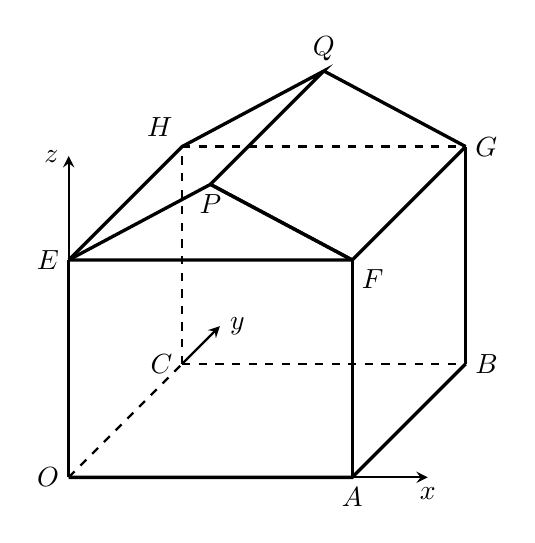
\begin{tikzpicture}[scale=1.2, >=stealth]
    % Định nghĩa tọa độ các đỉnh chính
    % Đáy OABC
    \coordinate (O) at (0, 0);
    \coordinate (A) at (3, 0);
    \coordinate (B) at (4.2, 1.2);
    \coordinate (C) at (1.2, 1.2);

    % Tầng hộp OABC.EFGB (EFGH)
    \coordinate (E) at (0, 2.3);
    \coordinate (F) at (3, 2.3);
    \coordinate (G) at (4.2, 3.5);
    \coordinate (H) at (1.2, 3.5);

    % Đỉnh mái nhà P và Q
    \coordinate (P) at (1.5, 3.1);
    \coordinate (Q) at (2.7, 4.3);

    % --- Các đường khuất (nét đứt) ---
    \draw[thick, dashed] (O) -- (C);
    \draw[thick, dashed] (C) -- (B);
    \draw[thick, dashed] (C) -- (H);
    \draw[thick, dashed] (H) -- (G);

    % --- Các đường nhìn thấy (nét liền) ---
    % Khung hình hộp chữ nhật
    \draw[very thick] (O) -- (A) -- (B);
    \draw[very thick] (O) -- (E);
    \draw[very thick] (A) -- (F);
    \draw[very thick] (B) -- (G);
    \draw[very thick] (E) -- (F) -- (G);

    % Mái nhà (mặt nghiêng & nóc mái)
    \draw[very thick] (E) -- (P) -- (F);
    \draw[very thick] (E) -- (H) -- (Q) -- (P);
    \draw[very thick] (F) -- (P);
    \draw[very thick] (G) -- (Q);

    % --- Các trục tọa độ Oxyz ---
    % Trục Ox
    \draw[thick, ->] (A) -- (3.8, 0) node[below] {$x$};
    % Trục Oy
    \draw[thick, ->] (C) -- (1.6, 1.6) node[right] {$y$};
    % Trục Oz
    \draw[thick, ->] (E) -- (0, 3.4) node[left] {$z$};

    % --- Đặt nhãn cho các điểm ---
    \node[left] at (O) {$O$};
    \node[below] at (A) {$A$};
    \node[right] at (B) {$B$};
    \node[left] at (C) {$C$};
    \node[left] at (E) {$E$};
    \node[below right] at (F) {$F$};
    \node[right] at (G) {$G$};
    \node[above left] at (H) {$H$};
    \node[below] at (P) {$P$};
    \node[above] at (Q) {$Q$};

\end{tikzpicture}
\end{center}
}{
    \textbf{a)} & Tọa độ của vectơ \(\vec{CF}\) là \((-6; 8; -4)\).
    & \textcolor{amberorange}{$\bigcirc$} & \textcolor{amberorange}{$\bigcirc$} \\ \hline
    
    \textbf{b)} & Chiều cao của kho hàng, tức khoảng cách từ điểm cao nhất của mái nhà đến mặt sàn bằng 7m.
    & \textcolor{amberorange}{$\bigcirc$} & \textcolor{amberorange}{$\bigcirc$} \\ \hline
    
    \textbf{c)} & Góc giữa mặt phẳng \((PQHE)\) và mặt phẳng \((OCGF)\) bằng \(80^\circ\) (kết quả làm tròn đến hàng đơn vị của độ).
    & \textcolor{amberorange}{$\bigcirc$} & \textcolor{amberorange}{$\bigcirc$} \\ \hline
    
    \textbf{d)} & Người ta cần sơn toàn bộ bề mặt bên ngoài của ngôi nhà (không gồm sàn nhà, gồm tất cả các mặt ngoài của mái nhà). Biết rằng giá sơn là 70 000 đồng/m\(^2\), khi đó tổng chi phí cần dùng để sơn toàn bộ bề mặt bên ngoài của ngôi nhà là 13,85 triệu đồng (kết quả làm tròn đến hàng phần trăm của triệu đồng).
    & \textcolor{amberorange}{$\bigcirc$} & \textcolor{amberorange}{$\bigcirc$} \\
}

% --- CÂU 16 ---
\questionTrueFalse{0}{16}{Trong không gian với hệ tọa độ \(Oxyz\), biết mặt đất là mặt phẳng \((Oxy)\), một cabin cáp treo xuất phát tại điểm \(A(10; 3; 0)\) và chuyển động đều theo đường cáp có vectơ chỉ phương là \(\vec{u} = (2; -2; 1)\) với tốc độ là \(4,5\) m/s (đơn vị trên mỗi trục tọa độ là mét).

\begin{figure}[H]
    \centering
    
\includegraphics[width=0.4\textwidth]{images/Cau16.png}
\end{figure}

}{
    \textbf{a)} & Cáp treo chuyển động trên đường thẳng có phương trình là: \(\begin{cases} x = 10 + 2k \\ y = 3 - 2k \\ z = k \end{cases} (k \in \mathbb{R})\).
    & \textcolor{amberorange}{$\bigcirc$} & \textcolor{amberorange}{$\bigcirc$} \\ \hline
    
    \textbf{b)} & Giả sử sau thời gian \(t(s)\) (\(t \geq 0\)) kể từ lúc xuất phát, cabin đến điểm \(M\). Khi đó tọa độ điểm \(M\) là \(M\left( 3t + 10; -3t + 3; \dfrac{3t}{2} \right)\).
    & \textcolor{amberorange}{$\bigcirc$} & \textcolor{amberorange}{$\bigcirc$} \\ \hline
    
    \textbf{c)} & Cabin dừng ở điểm \(B\) có hoành độ 550, khi đó cáp treo đã đi được quãng đường dài 800m.
    & \textcolor{amberorange}{$\bigcirc$} & \textcolor{amberorange}{$\bigcirc$} \\ \hline
    
    \textbf{d)} & Đường cáp tạo với mặt đất một góc \(19^\circ\) (kết quả làm tròn đến hàng đơn vị).
    & \textcolor{amberorange}{$\bigcirc$} & \textcolor{amberorange}{$\bigcirc$} \\
}

\newpage

\textit{\textbf{Phần III: Thí sinh trả lời từ câu 17 đến câu 22.}}

\vspace{0.3cm}
% --- CÂU 17 ---
\questionShortAnswer{0}{17}{Một quả bóng rổ được đặt ở một góc của căn phòng hình hộp chữ nhật, sao cho quả bóng chạm và tiếp xúc với hai bức tường và nền nhà của căn phòng đó thì có một điểm trên quả bóng có khoảng cách lần lượt đến hai bức tường và nền nhà là 17 cm, 18 cm, 21 cm (tham khảo hình minh họa). Hỏi độ dài đường kính của quả bóng bằng bao nhiêu cm biết rằng quả bóng rổ tiêu chuẩn có đường kính từ 23 cm đến 24,5 cm (kết quả làm tròn đến hàng phần chục)?
\begin{figure}[H]
    \centering
    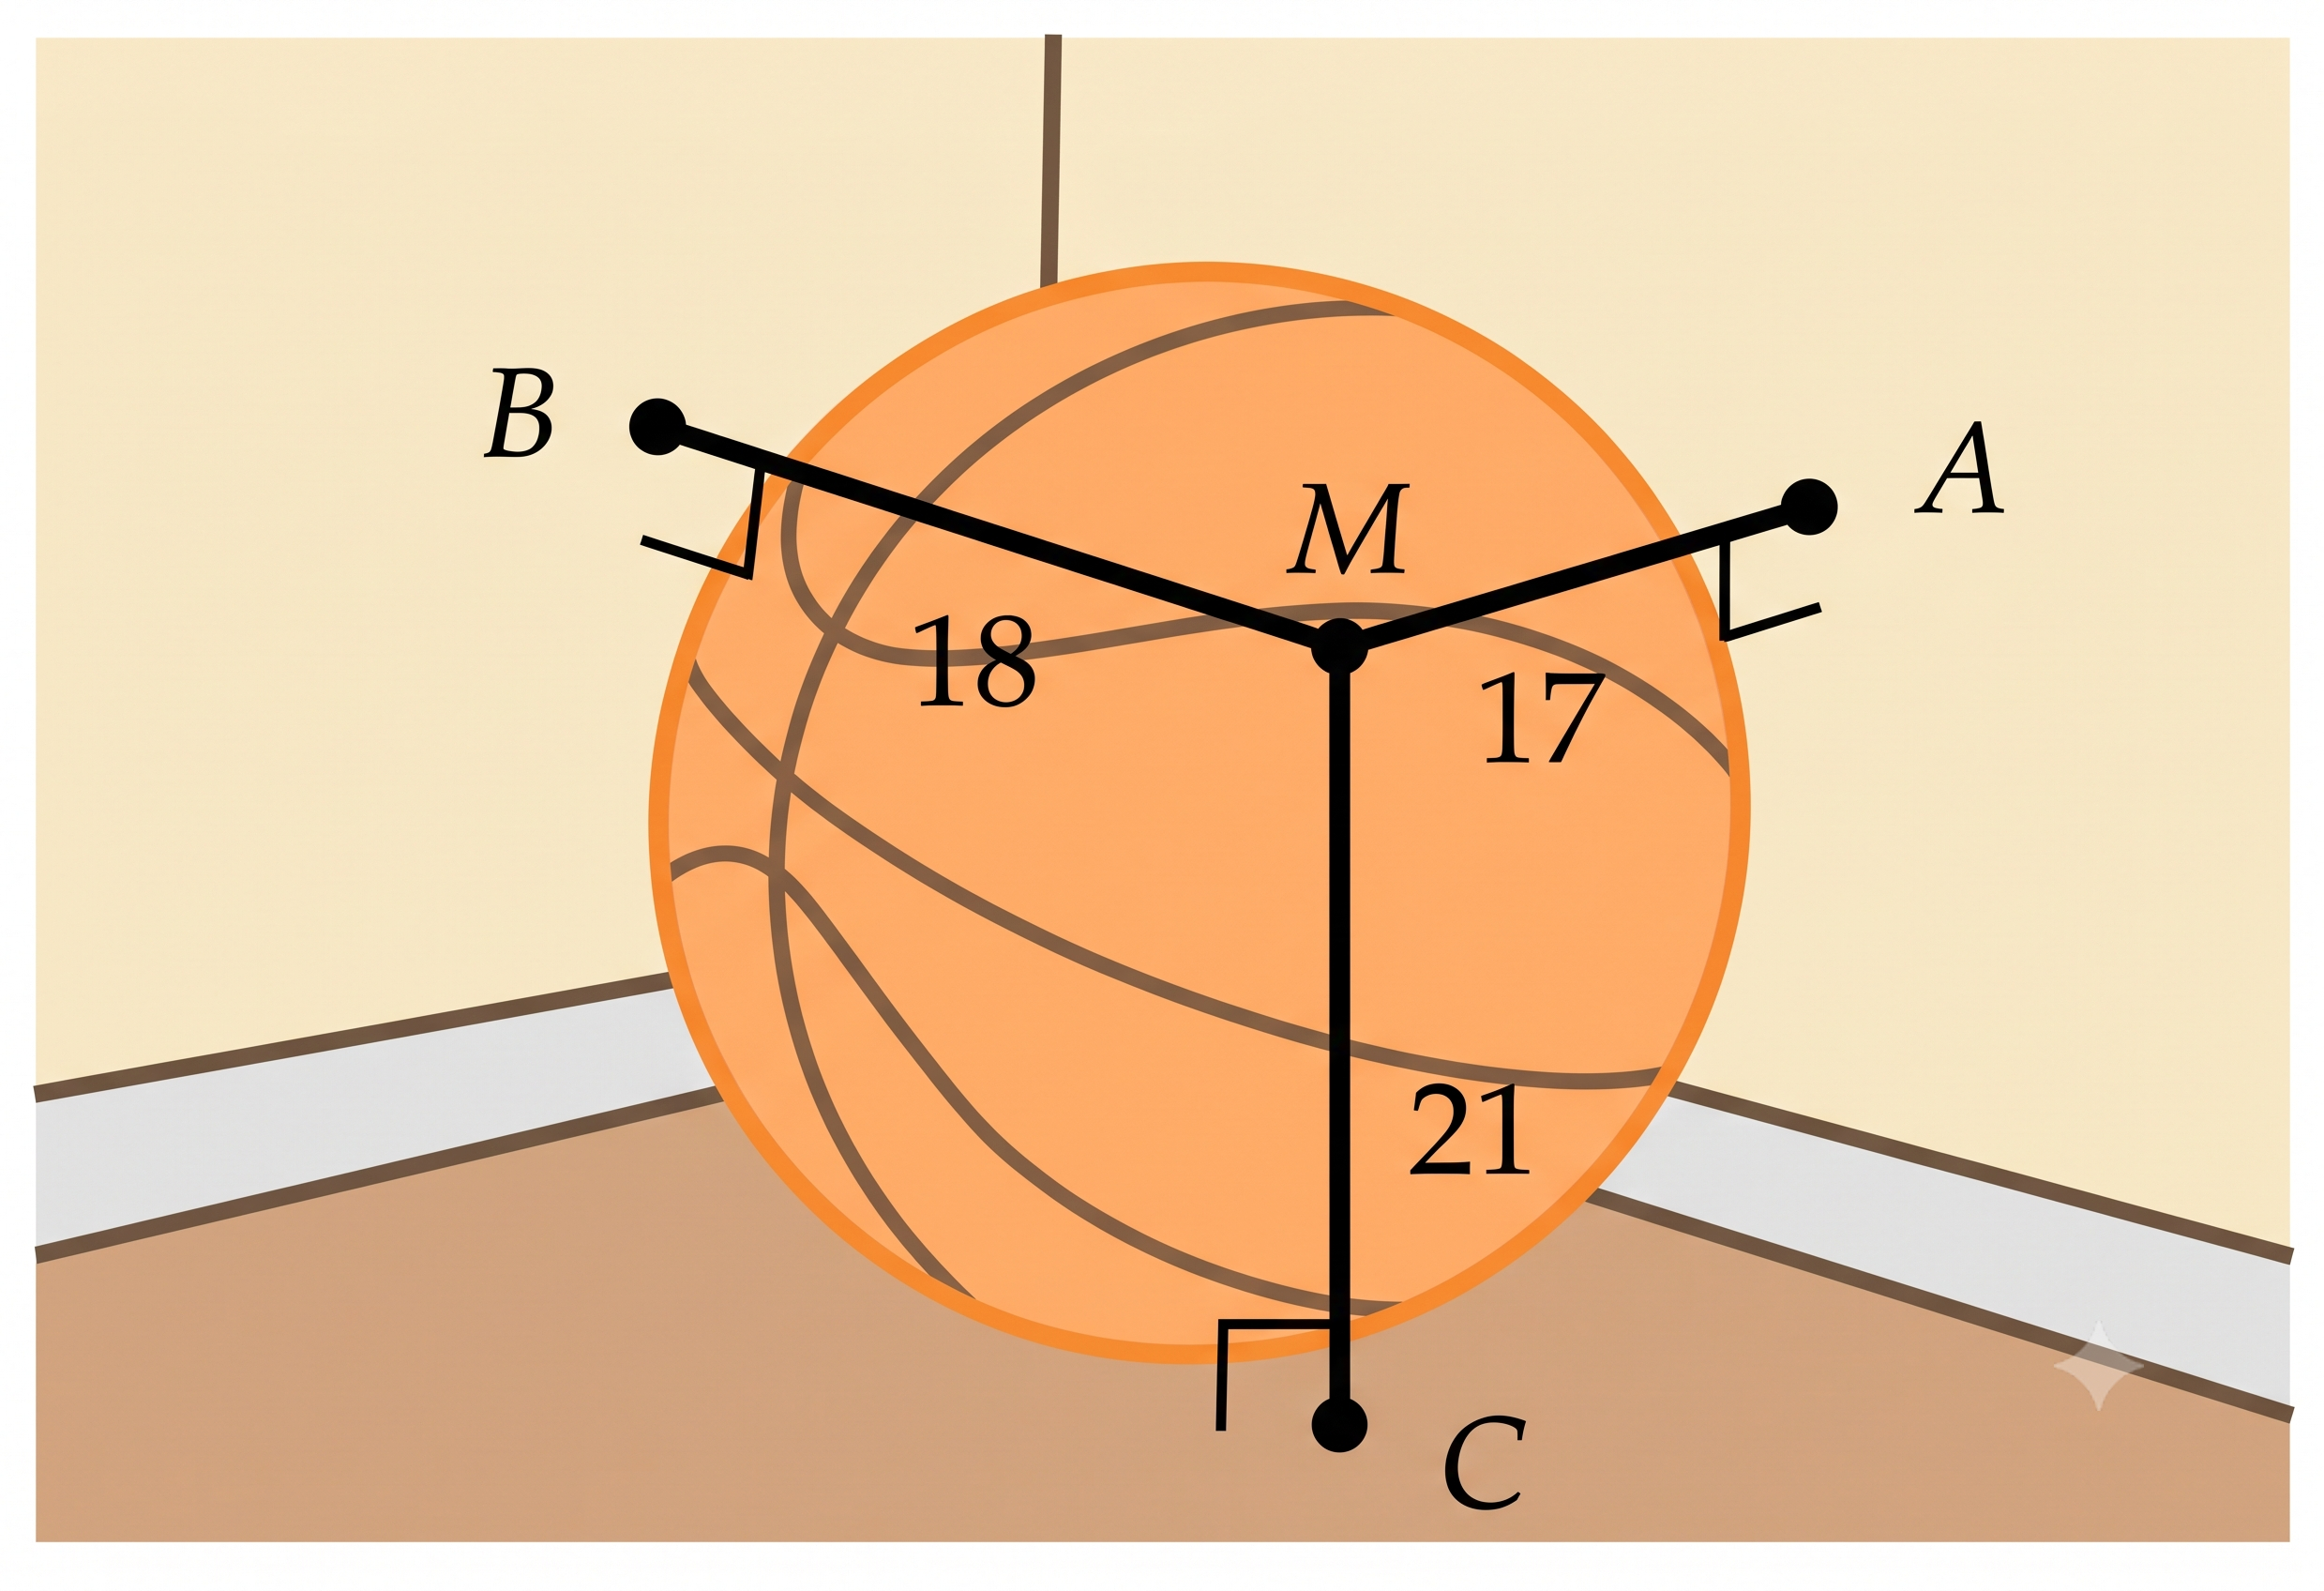
\includegraphics[width=0.3\textwidth]{images/Cau17.png}
\end{figure}

}

% --- CÂU 18 ---
\questionShortAnswer{0}{18}{Một công trình đang xây dựng được gắn hệ trục \(Oxyz\) (đơn vị trên mỗi trục tọa độ là mét). Ba bức tường lần lượt thuộc các mặt phẳng \((P), (Q), (R)\) (như hình vẽ) của tòa nhà lần lượt có phương trình:
\((P): 2x + 2y - 4z + 15 = 0\), \((Q): x + y + z - 12 = 0\), \((R): x + y - 2z = 0\).
Độ rộng của bức tường thuộc mặt phẳng \((Q)\) của tòa nhà bằng bao nhiêu mét (kết quả làm tròn đến chữ số hàng phần chục)?

\begin{figure}[H]
    \centering
    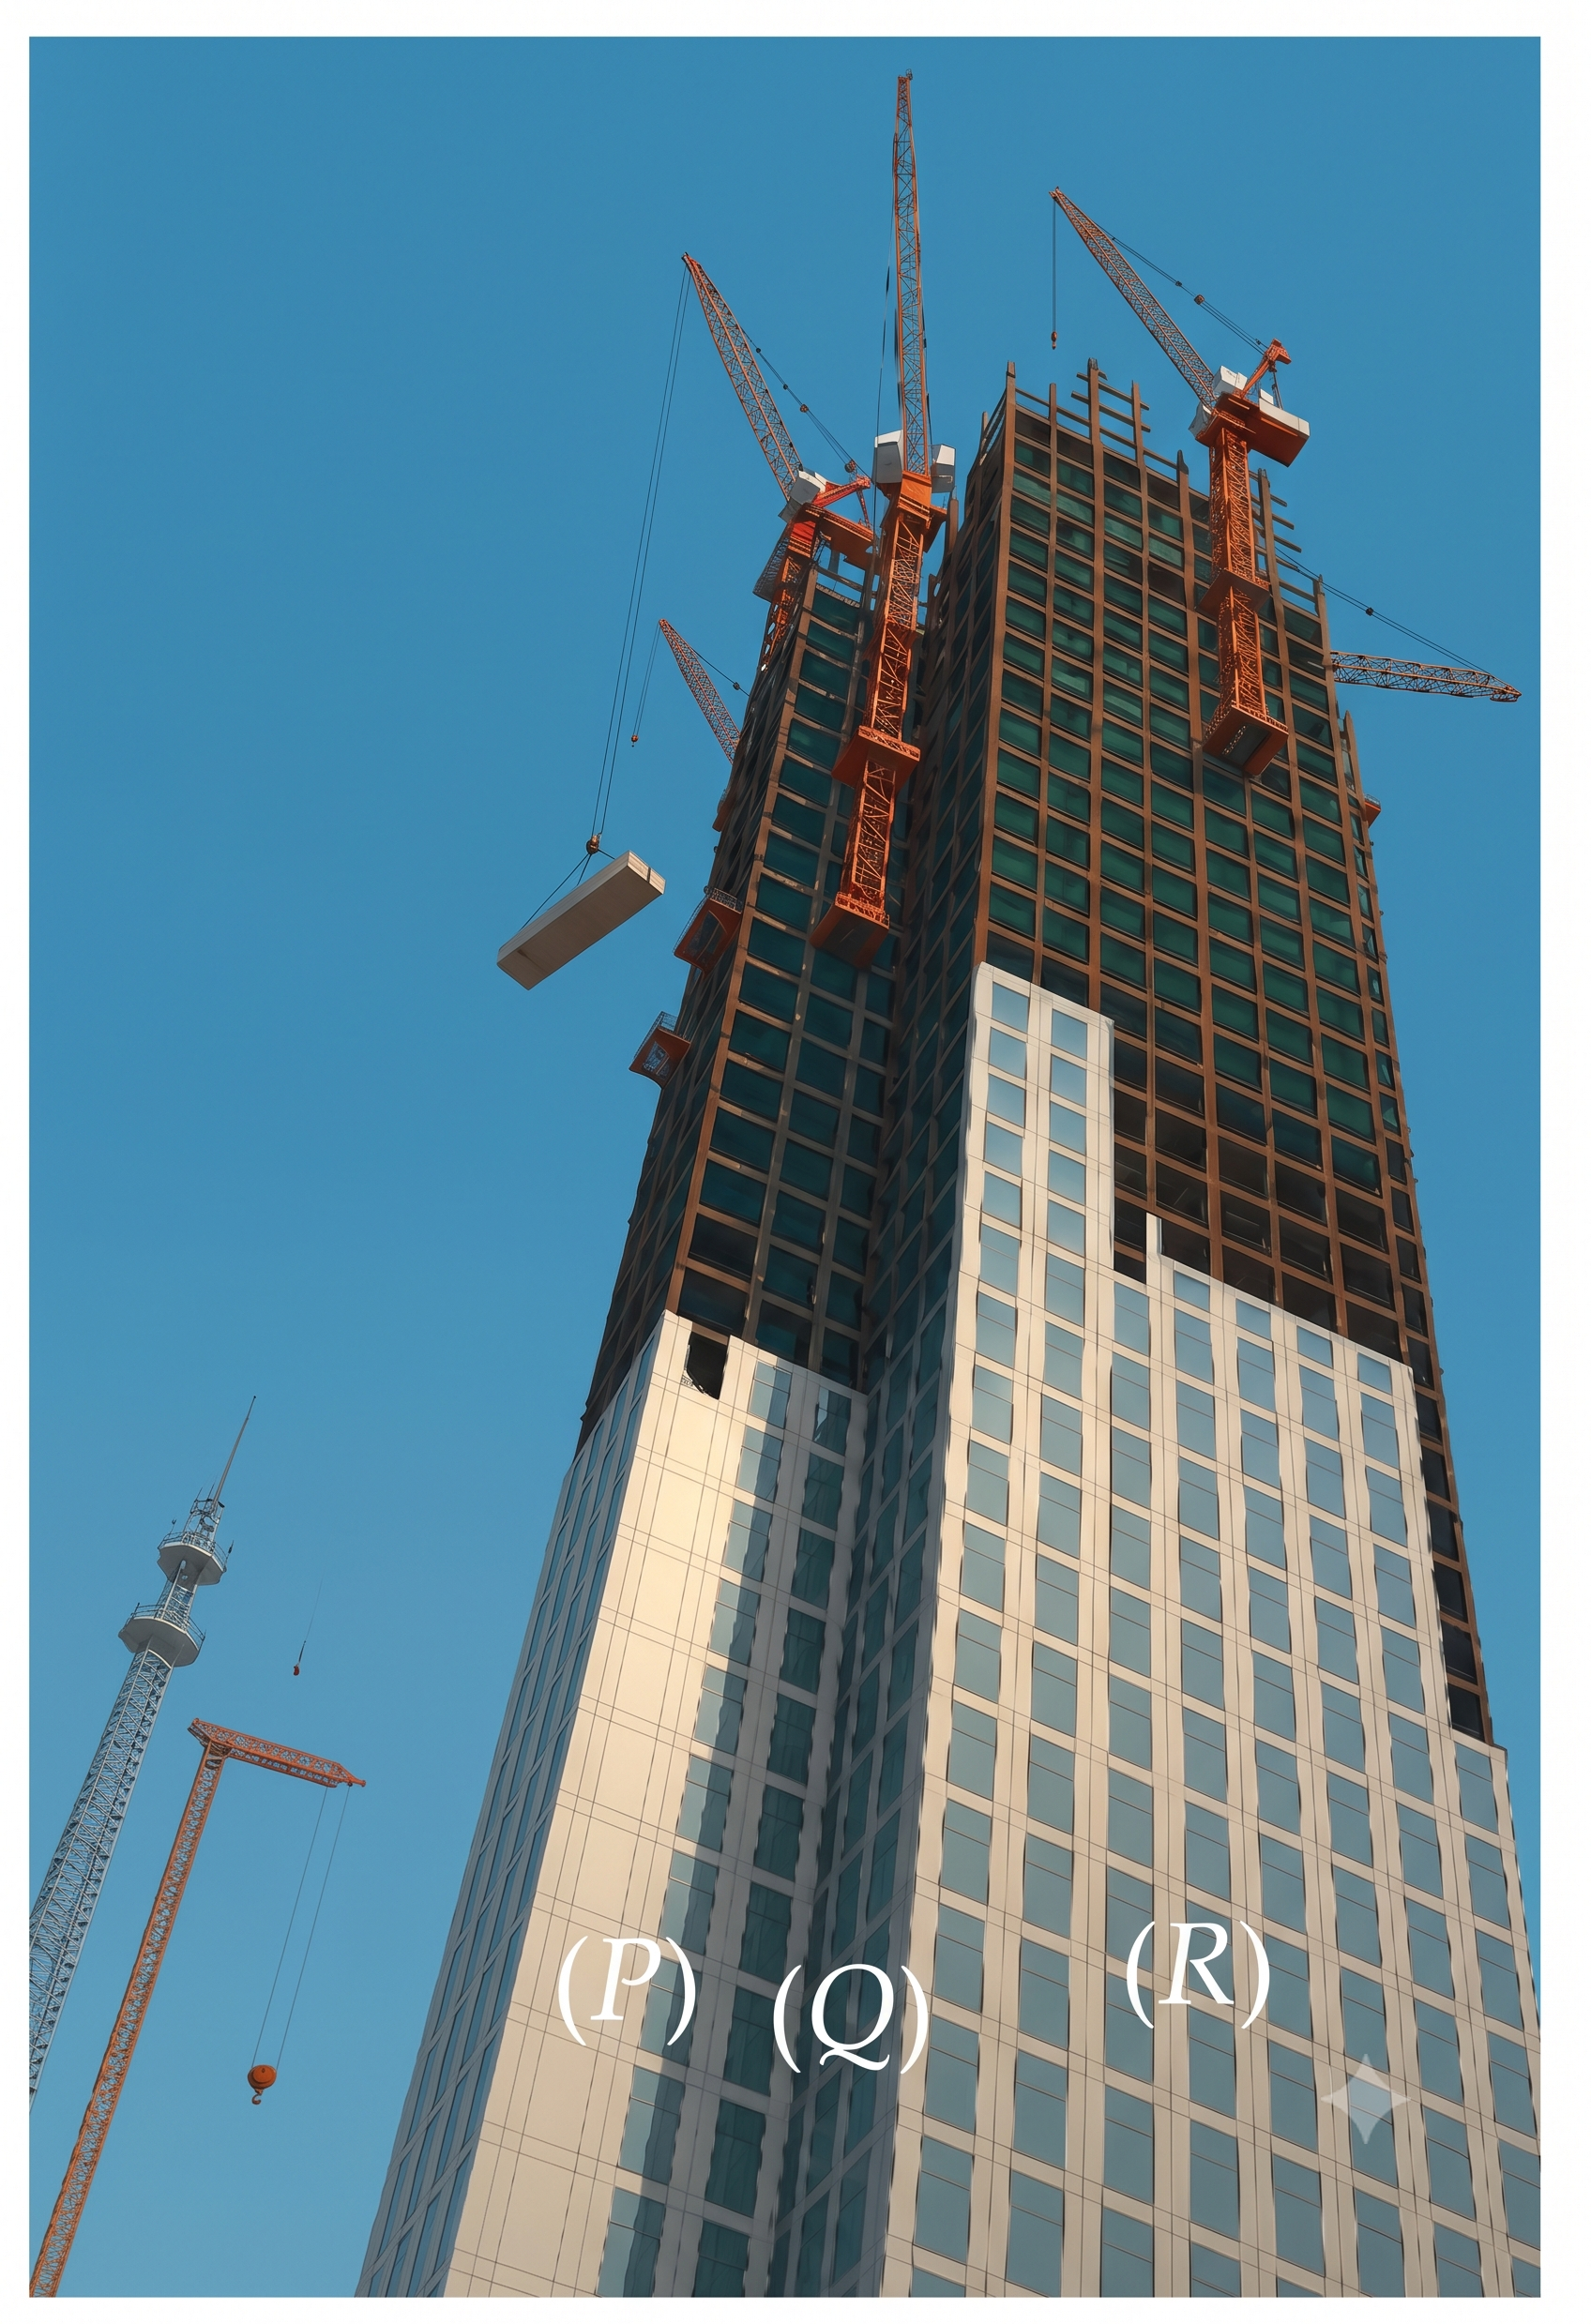
\includegraphics[width=0.3\textwidth]{images/Cau18.png}
\end{figure}

}

% --- CÂU 19 ---
\questionShortAnswer{0}{19}{Trong không gian \(Oxyz\), đài kiểm soát không lưu sân bay có tọa độ \(O(0; 0; 0)\), đơn vị trên mỗi trục tính theo kilômét. Một máy bay chuyển động hướng về đài kiểm soát không lưu qua hai vị trí \(A(-500; -250; 150)\), \(B(-200; -200; 100)\). Khi máy bay ở gần đài kiểm soát nhất, tọa độ của vị trí máy bay là \((a; b; c)\). Giá trị của biểu thức \(38a - 19b - 19c\) là bao nhiêu?
}

% --- CÂU 20 ---
\questionShortAnswer{0}{20}{Trong không gian \(Oxyz\), cho hai đường thẳng \(d: \dfrac{x+2}{1} = \dfrac{y-1}{-1} = \dfrac{z+1}{-2}\), \(\Delta: \dfrac{x-1}{2} = \dfrac{y+1}{1} = \dfrac{z-3}{1}\). Gọi \(M, N\) là hai điểm lần lượt thuộc đường thẳng \(d, \Delta\) sao cho góc giữa \(OM\) và \(\Delta\) bằng \(\alpha\) thỏa mãn \(\cos\alpha = \dfrac{2}{3}\); góc giữa \(ON\) và \(d\) bằng \(60^\circ\). Biết \(M\) có tọa độ nguyên, tính độ dài \(MN\) (kết quả làm tròn đến hàng phần trăm).
}

% --- CÂU 21 ---
\questionShortAnswer{0}{21}{Cho hình chóp \(S.ABCD\) có cạnh bên \(SA\) vuông góc với mặt phẳng đáy, \(ABCD\) là hình vuông cạnh bằng 8. Gọi \(M\) là trung điểm của \(SC\). Biết khoảng cách từ điểm \(B\) đến mặt phẳng \((AMD)\) bằng \(4\sqrt{2}\). Tính thể tích khối chóp \(S.ABCD\) (kết quả làm tròn đến hàng đơn vị).
}

% --- CÂU 22 ---
\questionShortAnswer{0}{22}{Trong không gian \(Oxyz\), cho ba điểm \(A(-2; 0; 1)\), \(B(1; 3; 4)\), \(C(3; 5; 3)\). Gọi \((P): ax + y + bz + c = 0\) \((a, b, c \in \mathbb{Z})\) là mặt phẳng đi qua hai điểm \(A, B\) sao cho khoảng cách từ \(C\) đến \((P)\) bằng \(\sqrt{6}\). Tính khoảng cách từ điểm \(K(24; 25; 23)\) đến \((P)\) (kết quả làm tròn đến hàng phần chục).
}

\end{document}
%1A, 2C, 3B, 4A, 5D, 6C, 7C, 8A, 9D, 10A, 11B, 12D
%13:DDDS  , 14:DSDD , 15:SDSD  , 16:DDSD
%17: 23.9, 18: 3.1, 19: 3300, 20: 5.04, 21: 171, 22: 2.9